%
% Modo de operación OFB, capítulo de antecedentes.
% Proyecto Lovelace.
%

\subsubsection{\textit{Output Feedback} (OFB)}
\label{sec:ofb}

Este modo es muy similar al anterior (\gls{gl:cfb}), salvo que la
retroalimentación va directamente de la salida del cifrador a bloques. De esta
forma, nada que tenga que ver con el texto en claro llega al cifrado a bloques;
este solamente se la pasa cifrando una y otra vez el
\gls{gl:vector_de_inicializacion}.

\begin{figure}
  \centering
  \begin{subfigure}{0.45\textwidth}
    \begin{center}
      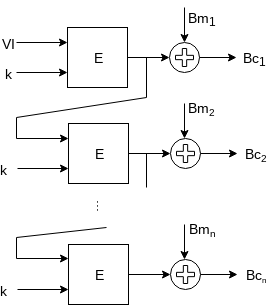
\includegraphics[width=0.7\linewidth]{diagramas/modo_ofb.png}
      \caption{Cifrado.}
    \end{center}
  \end{subfigure}
  \begin{subfigure}{0.45\textwidth}
    \begin{center}
      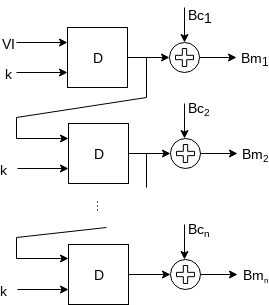
\includegraphics[width=0.7\linewidth]{diagramas/modo_ofb_inverso.png}
      \caption{Descifrado.}
    \end{center}
  \end{subfigure}
  \caption{\Gls{gl:modo_de_operacion} \gls{gl:ofb}.}
\end{figure}

\begin{pseudocodigo}[%
    caption={\Gls{gl:modo_de_operacion} \gls{gl:ofb}%
      (cifrado y descifrado).}%
    ]
    entrada: llave $ k $; vector de inicialización $ VI $;
             bloques de mensaje (cifrado o descifrado) $ Bm_1, Bm_2 \dots Bm_n $.
    salida:  bloques de mensaje (cifrado o descifrado) $ Bc_1, Bc_2 \dots Bc_n $.
    inicio
      auxiliar $\gets$ $ VI $
      para_todo $Bm$
        auxiliar $\gets$ E_k(auxiliar)
        $Bc_i$ $\gets$  auxiliar $\oplus$ $Bm_i$
      fin
      regresar $Bc$
    fin
\end{pseudocodigo}
